Nous avons tout d'abord découpé le projet en différentes tâches à réaliser afin de le mener à son terme. Voici un schéma représentant les principales étapes d'élaboration du projet.

\begin{center}
	\includegraphics[height=7cm]{images/Processus_DEV.png}\\
	\textit{Processus de développement utilisé au cours du projet}\\
\end{center}

\newpage
Nous avons choisi l'API three.JS car celle-ci permet de faire du WebGL de façon simple et facilite la mise en œuvre du projet. En effet, ce projet est notre premier contact avec le domaine du WebGL. De plus, nous avons repris le code d'un exemple de cette API.Cet exemple génère un monde virtuel avec le bruit de Perlin, qui rappelle le jeu vidéo Minecraft. Voici le rendu graphique de l'exemple :

\begin{center}
	\includegraphics[height=6cm]{images/threeJS_minecraft.png}\\
	\textit{Exemple du monde virtuel généré avec l'API three.JS}
	\footnote{Le code source de l'exemple de l'API three.JS se trouve là : \url{https://github.com/mrdoob/three.js/blob/master/examples/webgl_geometry_minecraft.html}}
\end{center}

Il a ensuite fallu adapter le projet afin de mettre le code source HTML, CSS, et JS dans des fichiers séparés.

\begin{center}
	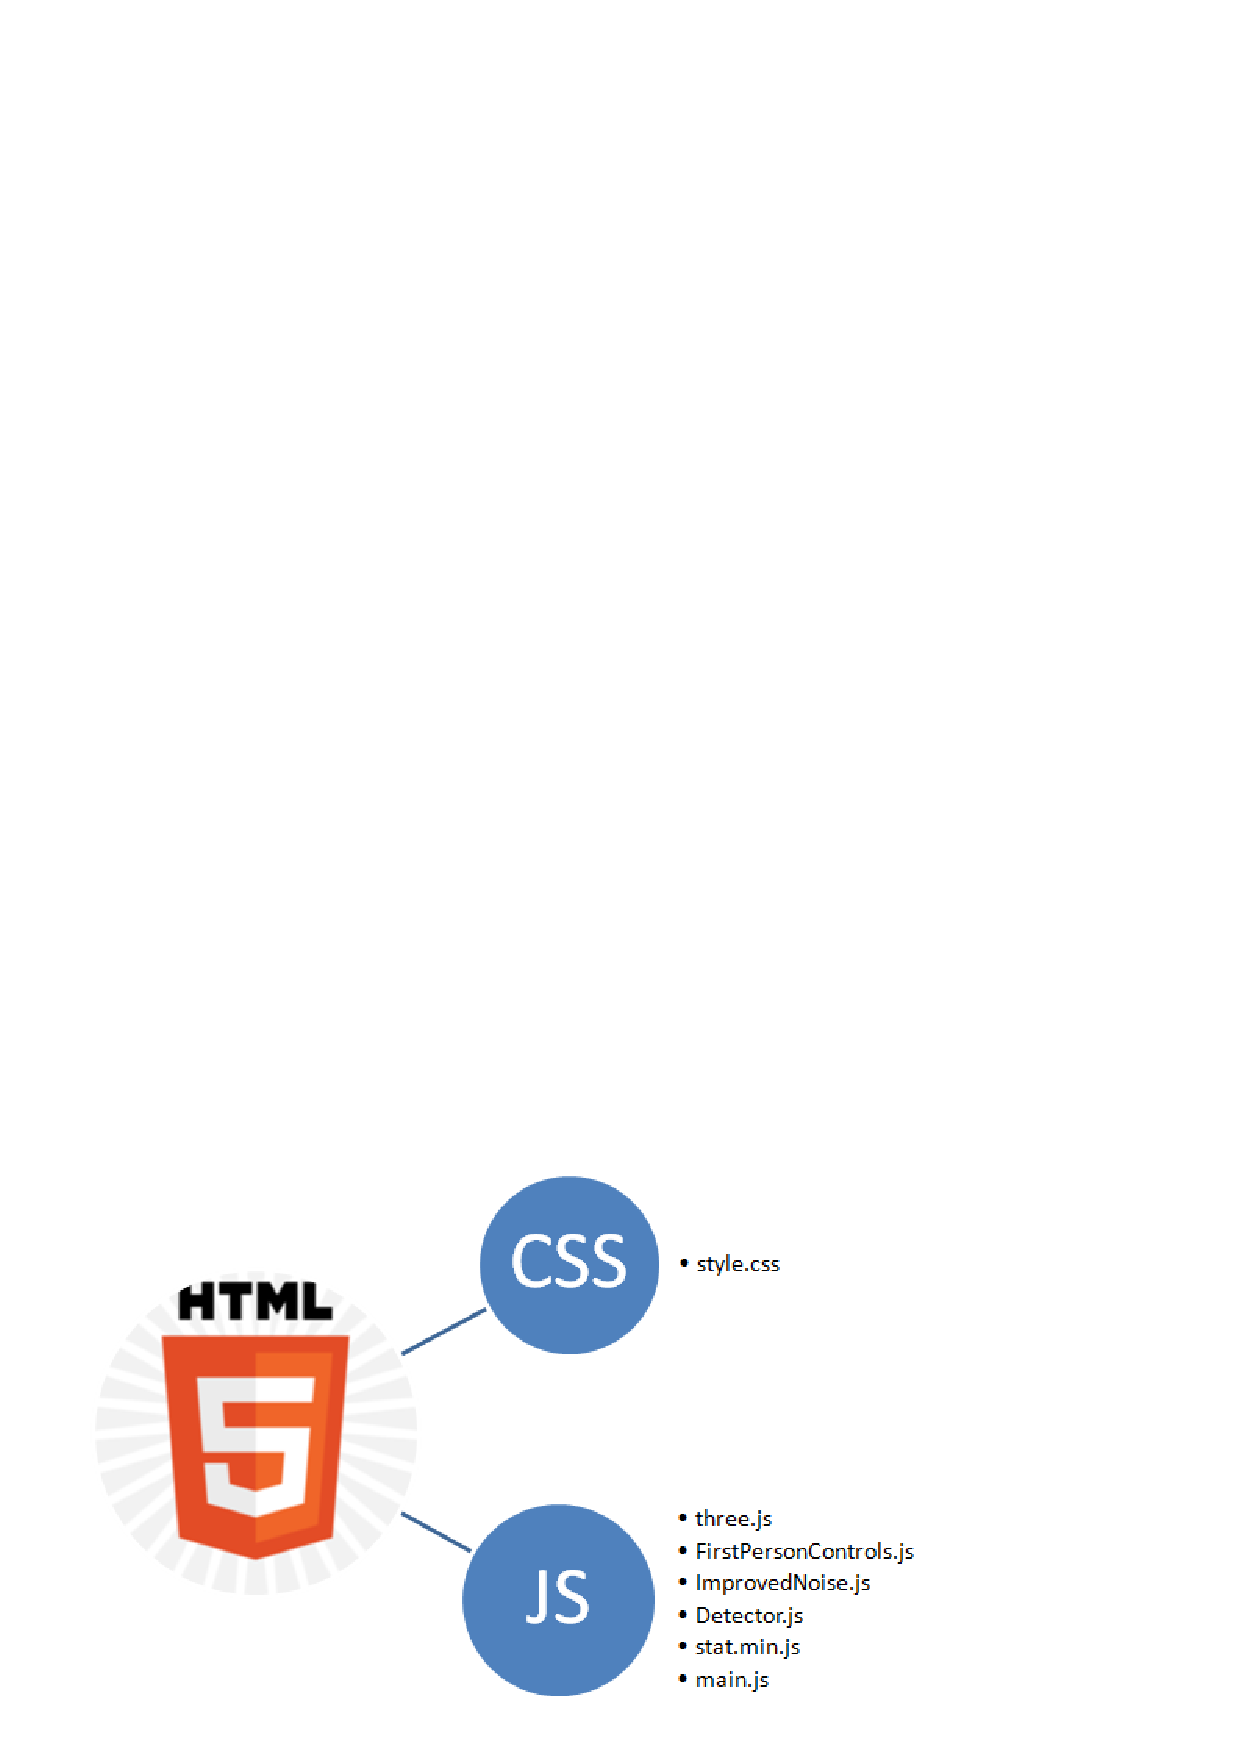
\includegraphics[height=6cm]{images/ProFileOrganisation.png}\\
	\textit{Structure du projet}
\end{center}